\documentclass[class=minimal,border=0pt, 11pt]{standalone}
\usepackage{xcolor}
\usepackage{amsmath, amsfonts, mathtools, amssymb, amsthm} 
\usepackage{tikz, pgfplots}
\pgfplotsset{compat=1.8}
\DeclareMathOperator{\parab}{par}
\definecolor{darkgreen}{rgb}{0.0 0.5 0.0}
\definecolor{whitegreen}{rgb}{0.0 0.75 0.0}
\definecolor{whiteblue}{rgb}{0.0 0.0 1.2}
\definecolor{darkred}{rgb}{0.8 0.0 0.0}
\def\samplepar{10}
\def\sampleatn{30}
\def\samplesamp{35}
\newcommand{\rosa}{\mathtt{Rosa}}
\newcommand{\fptaylor}{\mathtt{FPTaylor}}

\makeatletter
\newcommand*{\circled}{\@ifstar\circledstar\circlednostar}
\newcommand*{\squared}{\@ifstar\squaredstar\squarednostar}
\makeatother

\newcommand*\circledstar[1]{%
  \tikz[baseline=(C.base)]
    \node[%
      fill,
      circle,
      minimum size=1.em,
      text=white,
%      font=\sffamily,
      inner sep=0.5pt
    ](C) {\texttt{#1}};%
}
\newcommand*\circlednostar[1]{%
  \tikz[baseline=(C.base)]
    \node[%
      draw,
      circle,
      minimum size=1.em,
%      font=\sffamily,
      inner sep=0.5pt
    ](C) {\texttt{#1}};%
}
\newcommand*\squaredstar[1]{%
  \tikz[baseline=(C.base)]
    \node[%
      fill,
      rectangle,
      minimum size=1.em,
      text=white,
%      font=\sffamily,
      inner sep=0.5pt
    ](C) {\texttt{#1}};%
}
\newcommand*\squarednostar[1]{%
  \tikz[baseline=(C.base)]
    \node[%
      draw,
      rectangle,
      minimum size=1.em,
%      font=\sffamily,
      inner sep=0.5pt
    ](C) {\texttt{#1}};%
}

% argument #1: any options
\newenvironment{customlegend}[1][]{%
    \begingroup
    % inits/clears the lists (which might be populated from previous
    % axes):
    \csname pgfplots@init@cleared@structures\endcsname
    \pgfplotsset{#1}%
}{%
    % draws the legend:
    \csname pgfplots@createlegend\endcsname
    \endgroup
}%

% makes \addlegendimage available (typically only available within an
% axis environment):
\def\addlegendimage{\csname pgfplots@addlegendimage\endcsname}

%%--------------------------------

% definition to insert numbers
\pgfkeys{/pgfplots/number in legend/.style={%
        /pgfplots/legend image code/.code={%
            \node at (0.295,-0.0225){#1};
        },%
    },
}

\begin{document} 
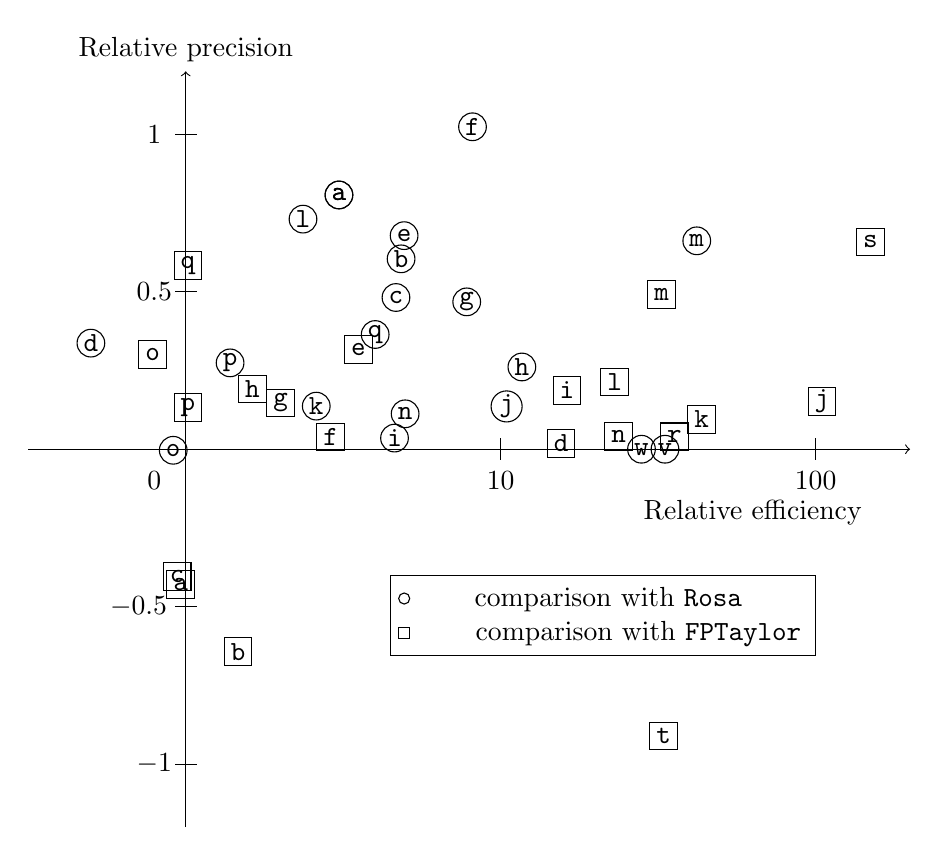
\begin{tikzpicture}[yscale=4, xscale=4]

\draw[->] (-0.5,0) -- (2.3,0) node[above] {}; \draw (1.8,-0.2) node {Relative efficiency}; 
\draw[->] (0,-1.2) -- (0,1.2) node[above] {Relative precision};

\draw (0.486569, 0.807273) node {\circled{a}}; 

\draw (0.486569, 0.807273) node {\circled{a}}; 
\draw (-0.016023, -0.429091) node {\squared{a}};

\draw (0.683855, 0.604478) node {\circled{b}}; 
\draw (0.166371, -0.643035) node {\squared{b}};

\draw (0.667619, 0.481752) node {\circled{c}}; 
\draw (-0.027079, -0.404380) node {\squared{c}};

\draw (-0.301030, 0.336842) node {\circled{d}}; 
\draw (1.191730, 0.018421) node {\squared{d}};

%\draw (0.693438, 0.628141) node {\circled{e}}; 
\draw (0.693438, 0.678141) node {\circled{e}}; 
\draw (0.547977, 0.316583) node {\squared{e}};

\draw (0.910589, 1.023739) node {\circled{f}}; 
\draw (0.460183, 0.038576) node {\squared{f}};

\draw (0.892205, 0.467890) node {\circled{g}}; 
\draw (0.301030, 0.146789) node {\squared{g}};

\draw (1.067347, 0.261146) node {\circled{h}}; 
\draw (0.211930, 0.191083) node {\squared{h}};

\draw (0.662961, 0.035388) node {\circled{i}}; 
\draw (1.210494, 0.187215) node {\squared{i}};

\draw (1.018885, 0.135897) node {\circled{j}}; 
\draw (2.020203, 0.151282) node {\squared{j}};

\draw (0.414509, 0.136842) node {\circled{k}}; 
\draw (1.638212, 0.094737) node {\squared{k}};

\draw (0.372386, 0.730561) node {\circled{l}}; 
\draw (1.361728, 0.213382) node {\squared{l}};

\draw (1.622603, 0.661677) node {\circled{m}}; 
\draw (1.511047, 0.491018) node {\squared{m}};

\draw (0.696678, 0.112434) node {\circled{n}}; 

%\draw (1.424538, 0.041005) node {\squared{n}};
\draw (1.374538, 0.041005) node {\squared{n}};

\draw (-0.039615, -0.003333) node {\circled{o}}; 
\draw (-0.105343, 0.300000) node {\squared{o}};

\draw (0.140927, 0.274175) node {\circled{p}}; 
\draw (0.007179, 0.133106) node {\squared{p}};

\draw (0.601558, 0.364256) node {\circled{q}}; 
\draw (0.006965, 0.582538) node {\squared{q}};

%\draw (1.531479, 0.036364) node {\squared{r}};
\draw (1.551479, 0.039364) node {\squared{r}};

\draw (2.174157, 0.658098) node {\squared{s}};

\draw (1.517126, -0.910667) node {\squared{t}};

\draw (1.521703, 0.000000) node {\circled{v}}; 

%\draw (1.477121, 0.000000) node {\circled{w}}; 
\draw (1.447121, 0.000000) node {\circled{w}};


\begin{customlegend}[
legend entries={ % <= in the following there are the entries
comparison with $\rosa$,
 \hspace{0.65cm} comparison with $\fptaylor$
},
legend style={at={(2,-0.4)}}] % <= to define position and font legend
% the following are the "images" and numbers in the legend
\addlegendimage{black,fill=white,only marks, mark=o}
%\addlegendimage{black,fill=white,circle}
\addlegendimage{black,fill=white,only marks, mark=square}
%\addlegendimage{rectangle,  minimum size=1.em, inner sep=0.5pt }
\end{customlegend}

\if{


\draw (0.486569, 0.807273) node {\circled{a}}; 
\draw (-0.016023, -0.429091) node {\squared{a}};

\draw (0.683855, 0.604478) node {\circled{b}}; 
\draw (0.166371, -0.643035) node {\squared{b}};

\draw (0.667619, 0.481752) node {\circled{c}}; 
\draw (-0.027079, -0.404380) node {\squared{c}};

\draw (-1.489958, 0.336842) node {\circled{d}}; 
\draw (0.002802, 0.018421) node {\squared{d}};

\draw (0.138256, 0.628141) node {\circled{e}}; 
\draw (-0.007204, 0.316583) node {\squared{e}};

\draw (0.599009, 1.005882) node {\circled{f}}; 
\draw (0.148603, 0.029412) node {\squared{f}};

\draw (0.892205, 0.454545) node {\circled{g}}; 
\draw (0.301030, 0.136364) node {\squared{g}};

\draw (0.945925, 0.261146) node {\circled{h}}; 
\draw (0.090508, 0.191083) node {\squared{h}};

\draw (0.662961, 0.035388) node {\circled{i}}; 
\draw (1.210494, 0.187215) node {\squared{i}};

\draw (1.018885, 0.135897) node {\circled{j}}; 
\draw (1.492916, 0.148718) node {\squared{j}};

\draw (0.414509, 0.136842) node {\circled{k}}; 
\draw (0.997985, 0.089474) node {\squared{k}};

\draw (0.372386, 0.730561) node {\circled{l}}; 
\draw (1.361728, 0.213382) node {\squared{l}};

\draw (1.622603, 0.661677) node {\circled{m}}; 
\draw (1.511047, 0.491018) node {\squared{m}};

\draw (0.696678, 0.112434) node {\circled{n}}; 

% slightly modified for presentation purpose \draw (1.424538, 0.041005) node {\squared{n}};
\draw (1.374538, 0.041005) node {\squared{n}};

\draw (-0.039615, 0.000000) node {\circled{o}}; 
\draw (-0.105343, 0.304348) node {\squared{o}};

\draw (1.034472, 0.240310) node {\circled{p}}; 
\draw (0.900723, 0.102990) node {\squared{p}};

\draw (1.790888, 0.123596) node {\circled{q}}; 
\draw (1.196295, 0.303371) node {\squared{q}};


% slightly modified for presentation purpose \draw (1.531479, 0.036364) node {\squared{r}};
\draw (1.551479, 0.039364) node {\squared{r}};

\draw (2.174157, 0.658098) node {\squared{s}};

\draw (1.614036, -0.965195) node {\squared{t}};

\draw (1.521703, 0.000000) node {\circled{v}}; 

% slightly modified for presentation purpose \draw (1.477121, 0.000000) node {\circled{w}}; 
\draw (1.447121, 0.000000) node {\circled{w}}; 

}\fi

\draw (-0.1,-0.1) node {$0$}; 
\draw (1,1pt) -- (1,-1pt); \draw (1,-0.1) node {$10$}; 
\draw (2,1pt) -- (2,-1pt); \draw (2,-0.1) node {$100$}; 

%\draw (-1,1pt) -- (-1,-1pt); \draw (-1,-0.1) node {$-10$}; 
%\draw (-2,1pt) -- (-2,-1pt); \draw (-2,-0.1) node {$-100$}; 

\draw (1pt,1) -- (-1pt,1); \draw (-0.1,1) node {$1$}; 
\draw (1pt,-1) -- (-1pt,-1); \draw (-0.1,-1) node {$-1$}; 
\draw (1pt,1/2) -- (-1pt,1/2); \draw (-0.1,1/2) node {$0.5$}; 
\draw (1pt,-1/2) -- (-1pt,-1/2); \draw (-0.15,-1/2) node {$-0.5$}; 
%\draw (2,1pt) -- (2,-1pt); \draw (2,-0.1) node {$100$}; 

%\draw (-1,1pt) -- (-1,-1pt); \draw (-1,-0.1) node {$-10$}; 
%\draw (-2,1pt) -- (-2,-1pt); \draw (-2,-0.1) node {$-100$}; 
\end{tikzpicture}
 \end{document}

\if{
let slog x = log (x) /. log(10.);;
let trel treal2float trosa tfptaylor = ((trosa)/.treal2float , ( tfptaylor )/.treal2float );;
let erel ereal2float erosa efptaylor = ((erosa -.ereal2float)/.ereal2float , (efptaylor -. ereal2float)/.ereal2float );;
let terel i ereal2float erosa efptaylor treal2float trosa tfptaylor = 
let a, b = trel treal2float trosa tfptaylor in 
let c, d = erel ereal2float erosa efptaylor in 
Printf.sprintf "
\\draw (%f, %f) node {\\circled{%c}}; 
\\draw (%f, %f) node {\\squared{%c}};
" 
(slog(a)) c i 
(slog(b)) d i;;

let s1 =  terel 'a' 2.75e-13  4.97e-13  1.57e-13 7.73  23.7  7.45 in
let s2 =  terel 'b' 8.04e-13  1.29e-12  2.87e-13 4.97  24.0  7.29 in
let s3 =  terel 'c' 1.37e-13  2.03e-13  8.16e-14 7.61  35.4  7.15 in
let s4 = terel 'd' 3.80e-13  5.08e-13  3.87e-13 0.40  0.20  6.22  in
let s5 = terel 'e' 3.98e-11  6.48e-11  5.24e-11 2.37  11.7  8.37  in
let s6 = terel 'f' 3.37e-16  6.82e-16  3.50e-16 1.22  9.93  3.52 in
let s7 = terel 'g' 1.09e-08  1.60e-08  1.25e-08 5.05  39.4  10.1 in
let s8 = terel 'h' 1.57e-16  1.98e-16  1.87e-16 3.10  36.2  5.05  in
let s9 = terel 'i' 8.76e-14  9.07e-14  1.04e-13 0.93  4.28  15.1 in
let s10 = terel 'j' 3.90e-13  4.43e-13  4.48e-13 3.15  32.9  98.0 in
let s11 = terel 'k' 1.90e-12  2.16e-12  2.07e-12 21.6  56.1  215.0 in
let s12 = terel 'l' 5.53e-16  9.57e-16  6.71e-16 0.42  0.99  9.66 in
let s13 = terel 'm' 6.68e-16  1.11e-15  9.96e-16 0.16  6.71  5.19 in
let s14 = terel 'n' 7.56e-16  8.41e-16  7.87e-16 0.38  1.89  10.1 in
let s15 = terel 'o' 3.00e-13  2.99e-13  3.90e-13 19.5  17.8  15.3 in
let s16 = terel 'p' 8.79e-16  1.12e-15  9.96e-16 1.80  2.49  1.83 in
let s17 = terel 'q' 7.33e-15  1.00e-14  1.16e-14 4.33  17.3  4.40 in
let s18 = terel 'r' 1.65e-15  0.  1.71e-15 0.06  0.  2.04 in
let s19 = terel 's' 7.78e-15  0.  1.29e-14 0.03  0.  4.48 in
let s20 = terel 't' 1.50e-13  0.  1.34e-14 1.90  0.  62.5  in
let s21 = terel 'v'   2.91 2.91 0. 0.37 12.3  0. in
let s22 = terel 'w'   2.01 2.01 0. 1.38 41.4 0. in
print_endline (s1^s2^s3^s4^s5^s6^s7^s8 ^ s9 ^ s10 ^ s11 ^ s12 ^ s13 ^s14^s15^s16^s17^s18^s19^s20^s21^s22);;

}\fi
